\pdfinfo{
	/ModDate (\pdfcreationdate)
	/Creator (Joanna Maciak)
	/Producer (pdfLaTeX)
	/Title (Sprawozdanie)
}

\documentclass[oneside, a4paper,11pt]{book}

\usepackage{color}
\usepackage[utf8]{inputenc}
\usepackage{listings}
\usepackage{fancyhdr}
\pagestyle{fancy}
\usepackage[breaklinks]{hyperref} 

\usepackage{pracadok}
\usepackage{longtable}
\usepackage[T1]{fontenc}
\usepackage{mathptmx}
\usepackage{caption}
\usepackage{subcaption}
\usepackage[labelfont=it]{caption}
\usepackage{graphicx}
\usepackage{sidecap}
\usepackage{wrapfig}
\usepackage{array}
\usepackage{amssymb}
\usepackage{geometry}
\usepackage{caption}
%\usepackage[justification=centering]{caption}
\newcolumntype{L}[1]{>{\raggedright\let\newline\\\arraybackslash\hspace{0pt}}m{#1}}
\newcolumntype{C}[1]{>{\centering\let\newline\\\arraybackslash\hspace{0pt}}m{#1}}
\newcolumntype{R}[1]{>{\raggedleft\let\newline\\\arraybackslash\hspace{0pt}}m{#1}}


\captionsetup{font=normalsize,labelfont={it}, labelsep = period}

\linespread{1.3}
\definecolor{mygray}{rgb}{0.5,0.5,0.5}
\definecolor{lightgray}{rgb}{0.9,0.9,0.9}
\definecolor{myorange}{rgb}{0.199,0.60,0.7}
\definecolor{newgray}{gray}{0.9}
\lstset{
	basicstyle=\linespread{1}\footnotesize,
	keywordstyle=\color{black}\bfseries,
	identifierstyle=\color{black},
	keywordstyle=\bfseries\color{myorange},
	commentstyle=\itshape\color{mygray},
	stringstyle=\ttfamily,
	showstringspaces=false,
	numbers=left, 
	numberstyle=\tiny, 
	stepnumber=1,
	numbersep=5pt,
	language=Java,
	tabsize=1,
	backgroundcolor=\color{lightgray}
	}

\begin{document}
\newcommand{\sos}{\texttt{SOS}\xspace}
\rfoot{\thepage}
\thispagestyle{empty}
\setlength{\unitlength}{1mm}

	\begin{center}	
	
	\LARGE{\textbf{POLITECHNIKA WARSZAWSKA}}\\[9ex]
	\LARGE{WYDZIAŁ ELEKTRONIKI \\I TECHNIK INFORMACYJNYCH}\\
	\par\noindent\\[.18 \textheight]
	\textbf{\Large{ANALIZA ALGORYTMÓW MST II}}\\[18ex]
	\raggedleft
	\begin{minipage}[l]{6cm}
	\large{Autorzy: \\Joanna Maciak\\Kacper Dominik}\\[.1ex]\\[9ex]
	\end{minipage}

	\centering
	\normalsize{Prowadzący: dr inż. Sebastian Kozłowski }
	\vfill

\end{center}
\begin{center}
	\large{Warszawa 2018}
\end{center}



\fancyhead[R]{SPIS TREŚCI}
\fancyhead[L]{}
\fancyfoot[C]{\thepage}
\fancyfoot[R]{}
\tableofcontents
\chapter [Sprawozdzanie 1] {Założenia projektowe} 
Tematem projektu jest \textbf{przeprowadzenie eksperymentalnej analizy czasu wykonywania dwóch algorytmów wyznaczania najlżejszego drzewa rozpinającego dla różnych klas grafów}.

Wybranymi algorytmami, będącymi przedmiotem tematu niniejszego projektu, są:\\
-- Algorytm Kruskala\\
-- Algorytm Prima\\

Językiem programowania, wybranym do implementacji powyższych algorytmów jest język Java.
\chapter [Sprawozdzanie 2]{Opis i implementacja algorytmów} 
\fancyhead[C]{OPIS I IMPLEMENTACJA ALHGORYTMÓW}
\fancyhead[L]{}
\fancyhead[R]{}
\textbf{Problem (zdefiniowany na podstawie \cite{prim2}):}\\
Znalezienie takiego podzbioru krawędzi spójnego grafu nieskierowanego ważonego, który zapewnia połączenie każdego wierzchołka grafu z dowolnym innym i ponadto posiada najmniejszą możliwą sumę wag krawędzi. \\Taki podzbiór nie może zawierać żadnego cyklu, a zatem jest drzewem i musi zawierać dokładnie \emph{n-1} krawędzi dla grafu o \emph{n} wierzchołkach. Drzewo takie ze względu na minimalną sumę wag nazywane jest minimalnym drzewem rozpinającym.

\section{Algorytm Prima}
\textbf{Dane wejściowe:} \\ 
Spójny ważony graf nieskierowany, zawierający n wierzchołków, gdzie $n \geqslant 2$.\\
Graf jest reprezentowany przez macierz sąsiedztwa \emph{graph}, gdzie element \emph{graph[i][j]} reprezentuje wagę krawędzi łączącej wierzchołki \emph{i} oraz \emph{j}.\\

\subsection{Pseudokod zaimplementowanego algorytmu}
\begin{enumerate}
	\item Inicjalizacja
	\begin{itemize}
		\item Utwórz pusty zbiór zawierający krawędzie minimalnego drzewa rozpinającego: \\ \emph{minSpanningTree}.
		\item Zainicjalizuj pustą listę odwiedzonych wierzchołków: \emph{visitedVertices}.
		\item Utwórz pustą listę krawędzi incydentnych do odwiedzonych wierzchołków: \emph{adjacencyEdges}.
	\end{itemize}

	\item Losuj wierzchołek początkowy: \emph{startV}.
	\item Oznacz wierzchołek początkowy jako odwiedzony poprzez dodanie go do listy wierzchołków odwiedzonych \emph{visitedVertices}.
	\item Pobierz do zmiennej \emph{adjacencyEdges} posortowaną względem wag listę wszystkich krawędzi incydentnych do wierzchołka \emph{startV}.
	\item Dopóki lista \emph{visitedVertices} nie zawiera wszystkich wierzchołków grafu:
	\item[a.] Zainicjalizuj zmienną aktualnie rozpatrywanej krawędzi -- \emph{minEdge} -- poprzez pobranie najmniejszego elementu listy \emph{adjacencyEdges}.
	\item[b.1.] Jeśli lista odwiedzonych wierzchołków \emph{visitedVertices} nie zawiera jeszcze wierzchołka końcowego aktualnie rozpatrywanej krawędzi \emph{minEdge}:\\
	-- dodaj krawędź \emph{minEdge} do zbioru krawędzi minimalnego drzewa rozpinającego \emph{minSpanningTree}\\
	-- przypisz zmiennej \emph{startV} wartość wierzchołka końcowego krawędzi \emph{minEdge}\\
	-- oznacz wierzchołek końcowy krawędzi \emph{minEdge } jako odwiedzony \\
	-- usuń krawędź uwzględnioną w \emph{minSpanningTree} -- \emph{minEdge} -- z listy krawędzi incydentnych do odwiedzonych wierzchołków
	-- ustal aktualną listę nietworzących cyklu krawędzi incydentnych do wierzchołków odwiedzonych
	\item[b.2.] Jeśli lista odwiedzonych wierzchołków \emph{visitedVertices} zawiera już wierzchołek końcowy aktualnie rozpatrywanej krawędzi \emph{minEdge}:\\
	-- usuń krawędź tworzącą cykl z listy krawędzi incydentnych do odwiedzonych wierzchołków\\
\end{enumerate} 

%%%%%%%%%%%%%%%%%%%%%%%%%%%%%%%%%
\newpage
\subsection{Zasada działania zaimplementowanego algorytmu na przykładzie}
Poniżej znajduje się legenda oznaczeń wykorzystanych w opisie działania algorytmu na przykładzie.

\begin{figure}[htb!]
	\centering
	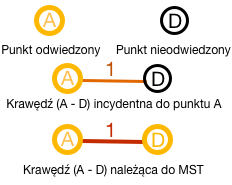
\includegraphics[width=0.4\textwidth]{tex/fig/legenda}
	\caption{Oznaczenia wykorzystane w opisie}
	\label{fig: legenda}
\end{figure}

Dany jest graf widoczny na rys.\ref{fig: g1}.  Wierzchołki oznaczono wielkimi literami alfabetu,\\ natomiast krawędziom nadano wagi $w\subseteq \{1,5\}$.\\

\begin{figure}[htb!]
	\centering
		
\includegraphics[width=0.4\textwidth]{tex/fig/graf1}
\caption{Graf wejściowy.}
\label{fig: g1}
\end{figure}

\textbf{Inicjalizacja}\\
Zbiór: \emph{minSpanningTree} =\{ \};\\
Lista wierzchołków odwiedzonych: \emph{visitedVertices} = [ ];\\
Lista krawędzi incydentnych: \emph{adjacencyEdges} = [ ];
\newpage
\textbf{Krok 1.}\\
Losowanie wierzchołka początkowego. W tym przypadku niech będzie to wierzchołek \textbf{A}.
\begin{center}
	\emph{startV} = A
\end{center}

\textbf{Krok 2.}\\
Oznaczenie wierzchołka \emph{startV} jako odwiedzony. 
\begin{figure}[htb!]
	\centering
	
\includegraphics[width=0.4\textwidth]{tex/fig/graf2}
	\caption{Prim -- Krok 2.}
	\label{fig: g2}
\end{figure}\\
Zbiór: \emph{minSpanningTree} =\{ \};\\
Lista wierzchołków odwiedzonych: \emph{visitedVertices} = [ A ];\\
Lista krawędzi incydentnych: \emph{adjacencyEdges} = [ ];\\

\textbf{Krok 3.}\\
Pobranie listy krawędzi incydentnych do wierzchołka \emph{startV}, które nie tworzą cyklu. 
\begin{figure}[htb!]
	\centering
	
\includegraphics[width=0.4\textwidth]{tex/fig/graf3}
	\caption{Prim -- Krok 3.}
	\label{fig: g3}
\end{figure}\\
Zbiór: \emph{minSpanningTree} =\{ \};\\
Lista wierzchołków odwiedzonych: \emph{visitedVertices} = [ A ];\\
Lista krawędzi incydentnych: \emph{adjacencyEdges} = [ (A -- D), (A -- B), (A -- C) ];\\

\textbf{Krok 4.}\\
Inicjalizacja \emph{minEdge} poprzez wybór pierwszego elementu posortowanej rosnąco listy krawędzi incydentnych \emph{adjacencyEdges}.\\
 \begin{center}
 	\emph{minEdge} = (A -- D)
 \end{center}

\textbf{Krok 5.}\\
Lista \emph{visitedVertices} nie zawiera jeszcze wierzchołka końcowego krawędzi \emph{minEdge} (D), dlatego:\\
-- Brak cyklu z krawędzią \emph{minEdge}\\
-- Dodanie krawędzi \emph{minEdge} do zbioru krawędzi minimalnego drzewa rozpinającego \emph{minSpanningTree}
 \begin{center}
Zbiór: \emph{minSpanningTree} =\{ (A -- D) \};
 \end{center}
-- przypisanie zmiennej \emph{startV} wartości wierzchołka końcowego krawędzi \emph{minEdge}
\begin{center}
	\emph{startV} = D
\end{center}
-- oznaczenie wierzchołka końcowego krawędzi \emph{minEdge } jako odwiedzony \\
-- usunięcie krawędzi uwzględnionej w \emph{minSpanningTree} -- \emph{minEdge} -- z listy krawędzi incydentnych do odwiedzonych wierzchołków \emph{adjacencyEdges}

\begin{center}
Lista wierzchołków odwiedzonych: \emph{visitedVertices} = [ A , D ];\\
Lista krawędzi incydentnych: \emph{adjacencyEdges} = [ (A -- B), (A -- C) ];\\
\end{center}
\begin{figure}[htb!]
	\centering
	
\includegraphics[width=0.4\textwidth]{tex/fig/graf4}
	\caption{Prim -- Krok 5.}
	\label{fig: g4}
\end{figure}
-- aktualizacja listy krawędzi incydentnych do odwiedzonych wierzchołków \emph{adjacencyEdges}
\begin{figure}[htb!]
	\centering
	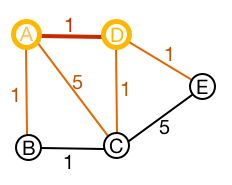
\includegraphics[width=0.4\textwidth]{tex/fig/graf5}
	\caption{Prim -- Krok 5 - aktualizacja listy krawędzi.}
	\label{fig: g5}
\end{figure}
\begin{center}
	Lista krawędzi incydentnych: \emph{adjacencyEdges} = [ (A -- B), (D -- C), (D -- E), (A -- C)];\\
\end{center}

\textbf{Krok 6.}\\
Aktualizacja \emph{minEdge} poprzez wybór pierwszego elementu posortowanej rosnąco listy krawędzi incydentnych \emph{adjacencyEdges}.\\
\begin{center}
	\emph{minEdge} = (A -- B)
\end{center}

\textbf{Krok 7.}\\
Lista \emph{visitedVertices} nie zawiera jeszcze wierzchołka końcowego krawędzi \emph{minEdge} (B), dlatego:\\
-- Brak cyklu z krawędzią \emph{minEdge}\\
-- Dodanie krawędzi \emph{minEdge} do zbioru krawędzi minimalnego drzewa rozpinającego \emph{minSpanningTree}
\begin{center}
	Zbiór: \emph{minSpanningTree} =\{ (A -- D), (A -- B) \};
\end{center}
-- przypisanie zmiennej \emph{startV} wartości wierzchołka końcowego krawędzi \emph{minEdge}
\begin{center}
	\emph{startV} = B
\end{center}
-- oznaczenie wierzchołka końcowego krawędzi \emph{minEdge } jako odwiedzony \\
-- usunięcie krawędzi uwzględnionej w \emph{minSpanningTree} -- \emph{minEdge} -- z listy krawędzi incydentnych do odwiedzonych wierzchołków \emph{adjacencyEdges}

\begin{center}
	Lista wierzchołków odwiedzonych: \emph{visitedVertices} = [ A , D , B];\\
	Lista krawędzi incydentnych: \emph{adjacencyEdges} = [ (D -- C), (D -- E), (A -- C) ];\\
\end{center}
\begin{figure}[htb!]
	\centering
	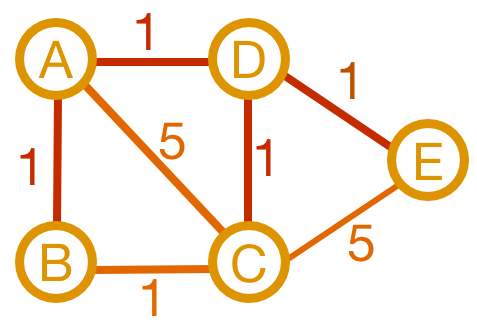
\includegraphics[width=0.4\textwidth]{tex/fig/graf6}
	\caption{Prim -- Krok 7.}
	\label{fig: g6}
\end{figure}
-- aktualizacja listy krawędzi incydentnych do odwiedzonych wierzchołków \emph{adjacencyEdges}
\begin{figure}[htb!]
	\centering
	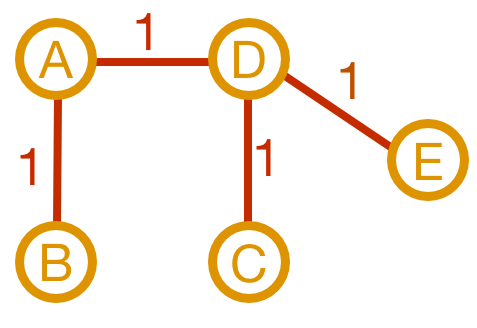
\includegraphics[width=0.4\textwidth]{tex/fig/graf7}
	\caption{Prim -- Krok 7 - aktualizacja listy krawędzi.}
	\label{fig: g7}
\end{figure}
\begin{center}
	Lista krawędzi incydentnych: \emph{adjacencyEdges} = [ (B -- C), (D -- C), (D -- E), (A -- C) ];\\
\end{center}

%%%%%%%%%%%%%%%%%%%%%%%%%%%%%%%%%%%%%%%%%%%%%%%%%%%%
\textbf{Krok 8.}\\
Aktualizacja \emph{minEdge} poprzez wybór pierwszego elementu posortowanej rosnąco listy krawędzi incydentnych \emph{adjacencyEdges}.\\
\begin{center}
	\emph{minEdge} = (B -- C)
\end{center}

\textbf{Krok 9.}\\
Lista \emph{visitedVertices} nie zawiera jeszcze wierzchołka końcowego krawędzi \emph{minEdge} (C), dlatego:\\
-- Brak cyklu z krawędzią \emph{minEdge}\\
-- Dodanie krawędzi \emph{minEdge} do zbioru krawędzi minimalnego drzewa rozpinającego \emph{minSpanningTree}
\begin{center}
	Zbiór: \emph{minSpanningTree} =\{ (A -- D), (A -- B), (B -- C) \};
\end{center}
-- przypisanie zmiennej \emph{startV} wartości wierzchołka końcowego krawędzi \emph{minEdge}
\begin{center}
	\emph{startV} = C
\end{center}
-- oznaczenie wierzchołka końcowego krawędzi \emph{minEdge } jako odwiedzony \\
-- usunięcie krawędzi uwzględnionej w \emph{minSpanningTree} -- \emph{minEdge} -- z listy krawędzi incydentnych do odwiedzonych wierzchołków \emph{adjacencyEdges}

\begin{center}
	Lista wierzchołków odwiedzonych: \emph{visitedVertices} = [ A , D , B, C];\\
	Lista krawędzi incydentnych: \emph{adjacencyEdges} = [ (D -- C), (D -- E), (A -- C) ];\\
\end{center}
\begin{figure}[htb!]
	\centering
	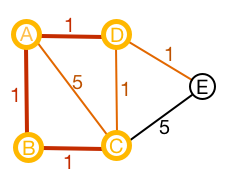
\includegraphics[width=0.4\textwidth]{tex/fig/graf8}
	\caption{Prim -- Krok 9.}
	\label{fig: g8}
\end{figure}
-- aktualizacja listy krawędzi incydentnych do odwiedzonych wierzchołków \emph{adjacencyEdges}
\begin{figure}[htb!]
	\centering
	
\includegraphics[width=0.4\textwidth]{tex/fig/graf9}
	\caption{Prim -- Krok 9 - aktualizacja listy krawędzi.}
	\label{fig: g9}
\end{figure}
\begin{center}
	Lista krawędzi incydentnych: \emph{adjacencyEdges} = [ (D -- C), (D -- E), (A -- C), (C -- E) ];\\
\end{center}
%%%%%%%%%%%%%%%%%%%%%%%%%%%%%%%%%%%%%%%%%%%%%%%%%%%%%%%%%%%%%%%%

\textbf{Krok 10.}\\
Aktualizacja \emph{minEdge} poprzez wybór pierwszego elementu posortowanej rosnąco listy krawędzi incydentnych \emph{adjacencyEdges}.\\
\begin{center}
	\emph{minEdge} = (D -- C)
\end{center}

\textbf{Krok 11.}\\
Lista \emph{visitedVertices} zawiera wierzchołek krawędzi \emph{minEdge} (C), dlatego:\\
-- Usunięcie krawędzi \emph{minEdge} z listy krawędzi incydentnych do odwiedzonych wierzchołków
\begin{center}
	Lista krawędzi incydentnych: \emph{adjacencyEdges} = [ (D -- E), (A -- C), (C -- E) ];
\end{center}

\begin{figure}[htb!]
	\centering
	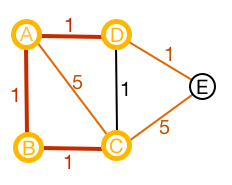
\includegraphics[width=0.4\textwidth]{tex/fig/graf10}
	\caption{Prim -- Krok 11.}
	\label{fig: g10}
\end{figure}
%%%%%%%%%%%%%%%%%%%%%%%%%%%%%%%%%%%%%%%%%%%%%%%%%%%%%%%%%%%%%%
\textbf{Krok 12.}\\
Aktualizacja \emph{minEdge} poprzez wybór pierwszego elementu posortowanej rosnąco listy krawędzi incydentnych \emph{adjacencyEdges}.\\
\begin{center}
	\emph{minEdge} = (D -- E)
\end{center}

\textbf{Krok 13.}\\
Lista \emph{visitedVertices} nie zawiera jeszcze wierzchołka końcowego krawędzi \emph{minEdge} (E), dlatego:\\
-- Brak cyklu z krawędzią \emph{minEdge}\\
-- Dodanie krawędzi \emph{minEdge} do zbioru krawędzi minimalnego drzewa rozpinającego \emph{minSpanningTree}
\begin{center}
	Zbiór: \emph{minSpanningTree} =\{ (A -- D), (A -- B), (B -- C), (D -- E) \};
\end{center}
-- przypisanie zmiennej \emph{startV} wartości wierzchołka końcowego krawędzi \emph{minEdge}
\begin{center}
	\emph{startV} = E
\end{center}
-- oznaczenie wierzchołka końcowego krawędzi \emph{minEdge } jako odwiedzony \\
-- usunięcie krawędzi uwzględnionej w \emph{minSpanningTree} -- \emph{minEdge} -- z listy krawędzi incydentnych do odwiedzonych wierzchołków \emph{adjacencyEdges}

\begin{center}
	Lista wierzchołków odwiedzonych: \emph{visitedVertices} = [ A , D , B, C, E];\\
	Lista krawędzi incydentnych: \emph{adjacencyEdges} = [ (C -- E), (A -- C) ];\\
\end{center}
-- aktualizacja listy krawędzi incydentnych do odwiedzonych wierzchołków \emph{adjacencyEdges}
\begin{figure}[htb!]
	\centering
	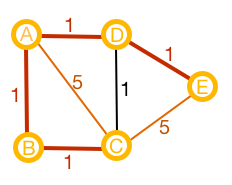
\includegraphics[width=0.4\textwidth]{tex/fig/graf11}
	\caption{Prim -- Krok 13.}
	\label{fig: g11}
\end{figure}
\begin{center}
	Lista krawędzi incydentnych: \emph{adjacencyEdges} = [ (C -- E), (A -- C) ];\\
\end{center}
\newpage
\textbf{Krok 14.}\\
Lista \emph{visitedVertices} zwiera wszystkie wierzchołki grafu wejściowego. W związku z tym otrzymano następujące drzewo rozpinające:\\
\begin{figure}[htb!]
	\centering
	
\includegraphics[width=0.4\textwidth]{tex/fig/graf12}
	\caption{Prim -- Krok 14 -- otrzymane MST.}
	\label{fig: g14}
\end{figure}
\newpage
\subsection{Składowe implementacji algorytmu}

\begin{table}[!hbp]
	\hspace{-60pt}
	\begin{tabular}{|C{5cm}|C{3cm}|C{9cm}|} \hline
		\textbf{Składowa}& \textbf{Rodzaj}& \textbf{Opis}\\ \hline
		rand & Zmienna pomocnicza  & Element odpowiedzialny za losowy wybór wierzchołka początkowego\\ \hline
		startV & Zmienna typu int  & Wierzchołek początkowy minimalnej krawędzi z listy \emph{adjacencyEdgesList}. Na początku przyjmuje wartość losową. \\ \hline
		visitedVertices & Lista elementów typu Integer  & Lista odwiedzonych wierzchołków grafu\\ \hline
		adjacencyEdgesList & Lista elementów typu Edge& Lista krawędzi incydentnych do odwiedzonych wierzchołków grafu\\
		&ArrayList<Edge>&\\ \hline
		minSpanningTree & Zbiór Set<Edge>  & Zbiór krawędzi, tworzących minimalne drzewo rozpinające\\ \hline
		minEdge & Zmienna typu Edge  & Obiekt klasy \emph{ Edge} (krawędź), zawierający minimalną krawędź  z listy \emph{adjacencyEdgesList} \\ \hline
		setVertexVisited(int vertex, ArrayList<Integer> list) & metoda & Metoda dodająca wierzchołek \emph{vertex} do listy wierzchołków odwiedzonych \emph{list} jeśli lista ta nie zawiera wierzchołka \emph{vertex}\\ \hline
		getAllAdjacencyEdges(int vertex, int[][] graph) & Metoda zwracająca listę obiektów Edge  & Metoda odpowiedzialna za ustalenie listy krawędzi incydentnych do odwiedzonych punktów \emph{adjacencyEdgesList}. Dla każdego wierzchołka \emph{i} $\subseteq V$ grafu weryfikuje czy dany wierzchołek \emph{i} tworzy krawędź z wierzchołkiem \emph{vertex}. Jeśli krawędź taka istnieje i lista \emph{visitedVertices} nie zawiera wierzchołka \emph{i}, to do listy \emph{adjacencyEdgesList} zostaje dodana krawędź (\emph{vertex} -- \emph{i})\\ \hline
		minSpanningTree.add(minEdge) & Operacja na zbiorze minSpanningTree & Operacja polegająca na dodaniu do zbioru \emph{minSpanningTree} minimalnej krawędzi \emph{minEdge}\\ \hline
	\end{tabular}
	\caption{Składowe implementacji algorytmu Prima}
	\label{skladowe}
\end{table}
\newpage
\begin{table}[!hbp]
	\hspace{-60pt}
	\begin{tabular}{|C{5cm}|C{3cm}|C{9cm}|} \hline
		\textbf{Składowa}& \textbf{Rodzaj}& \textbf{Opis}\\ \hline
		adjacencyEdges.remove(minEdge) & Operacja na liście \emph{adjacencyEdges} & Operacja polegająca na usunięciu z listy krawędzi \emph{adjacencyEdges} krawędzi \emph{minEdge}\\ \hline
		Edge & Klasa &Jest to klasa, której obiekty reprezentują krawędzie grafu. Ich atrybutami są: wierzchołek początkowy i końcowy krawędzi oraz jej waga. Klasa implementuje również metodę odpowiedzialną za sortowanie obiektów Edge znajdujących się w liście (metoda compareTo(Edge arg)) oraz metodę odpowiedzialną za wypisanie danej krawędzi (metoda toString()).\\ \hline
		
	\end{tabular}
	\caption{Składowe implementacji algorytmu Prima c.d.}
	\label{skladowe2}
\end{table}


\begin{center}
\textbf{Uwagi}
\end{center}
\begin{itemize}
\item W celu realizacji projektu zaistniała również konieczność implementacji modułu generującego macierz sąsiedztwa reprezentującą graf oraz zapisującego ją do pliku tekstowego na pulpicie. 
Ponadto należało zaimplementować mechanizm odpowiedzialny za odczyt wygenerowanej macierzy z pliku.
\item W procesie implementacji algorytmu Prima bazowano na następujących źródłach: \cite{prim} oraz \cite{prim3}. Źródła te miały wpływ na wybór odpowiednich struktur danych oraz na samo zrozumienie istoty algorytmu.
\end{itemize}


\newpage
\section{Algorytm Kruskala}
\subsection{Pseudokod opisujący działanie algorytmu Kruskala:}

\textbf{Inicjalizacja:}
\begin{enumerate}
	\item	Utwórz las L z wierzchołków oryginalnego grafu – każdy wierzchołek jest na początku osobnym drzewem.
	\item Utwórz posortowany zbiór S zawierający wszystkie krawędzie oryginalnego grafu.
\end{enumerate}

\begin{center}
	\textbf{Tworzenie MST}
\end{center}

\begin{enumerate}
\item Wybierz i usuń z S jedną z krawędzi o minimalnej wadze.
\item Jeśli krawędź ta łączyła dwa różne drzewa, to dodaj ją do lasu L tak, aby połączyła dwa odpowiadające drzewa w jedno.
\item W przeciwnym wypadku odrzuć ją.
\item Jeżeli wciąż istnieje więcej niż jedno drzewo przejdź do punktu 1.
\end{enumerate}

Po zakończeniu algorytmu L jest minimalnym drzewem rozpinającym zgodnie z \cite{gis}.

\newpage
\subsection{Działanie algorytmu na przykładzie}
Dany jest graf posiadający następujące składowe:
\begin{itemize}
\item Wierzchołki: {A}, {B}, {C}, {D}, {E}
\item Krawędzie: {A B, 1}, {A D, 1}, {C D, 1}, {D E, 1}, {B C, 1}, {A C, 5}, {C E, 5}
\end{itemize}

\textbf{Legenda oznaczeń w poniższym przykładzie:}\\
\begin{figure}[htb!]
	\centering
	
\includegraphics[width=0.3\textwidth]{tex/fig/Picture1}
	\caption{Oznaczenia wykorzystane w opisie algorytmu Kruskala}
	\label{fig: legendK}
\end{figure}

\begin{center}
	\textbf{Przebieg algorytmu}
\end{center}
\begin{enumerate}
	\item Pierwszy etap wykonania algorytmu - ustalenie zbioru wierzchołków S oraz zbioru krawędzi L:\\
	S: {A}, {B}, {C}, {D}, {E}
\\
	L: {A B}, {A D}, {C D}, {D E}, {B C}, {A C}, {C E}
\\
	\begin{figure}[htb!]
		\centering
		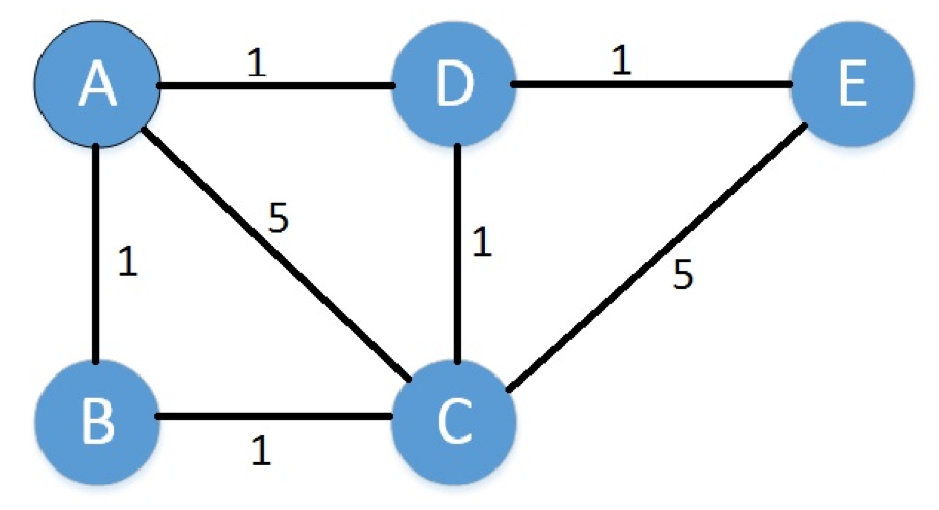
\includegraphics[width=0.4\textwidth]{tex/fig/Picture2}
		\caption{Przykładowy graf / pierwszy etap wykonania algorytmu Kruskala}
		\label{fig: legendK1}
	\end{figure}

\newpage
\item Krok 2\\
Ze zbioru S usunięta została jedna z krawędzi o najmniejszej wadze. {A B} Ponieważ wierzchołki, które łączyła znajdowały się w osobnych drzewach w L zostały połączone w jedno drzewo {A, B}, więc dodawana jest krawędź dodawana jest do W.\\
S: {A, B}, {C}, {D}, {E}
\\
L: {A D}, {C D}, {D E}, {B C}, {A C}, {C E}
\\
	\begin{figure}[htb!]
	\centering
	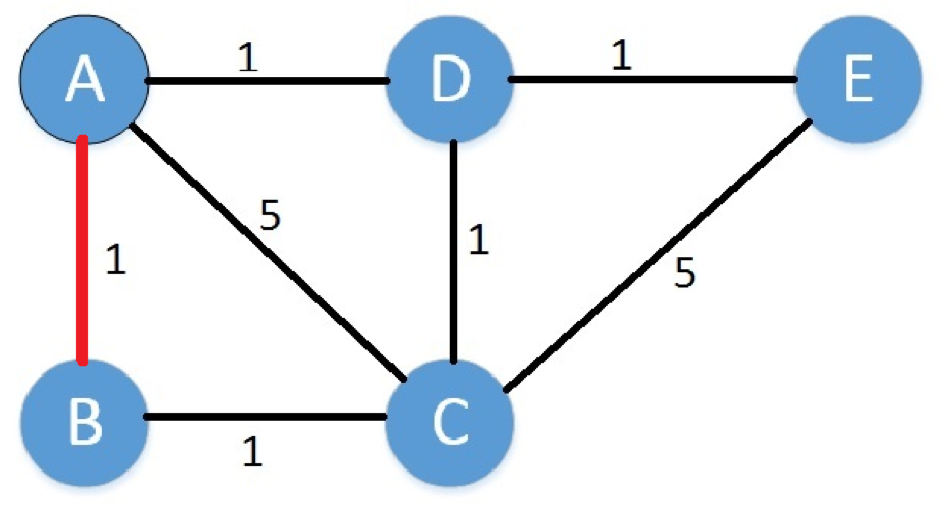
\includegraphics[width=0.4\textwidth]{tex/fig/Picture3}
	\caption{Drugi etap wykonania algorytmu Kruskala}
	\label{fig: legendK2}
\end{figure}

\item Krok 3\\
Ze zbioru S usunięta została jedna z krawędzi o najmniejszej wadze. {A D} Ponieważ wierzchołki, które łączyła znajdowały się w osobnych drzewach w L zostały połączone w jedno drzewo {A, B, D}, więc dodawana jest krawędź dodawana jest do W.\\
S: {A, B, D}, {C}, {E}
\\
L: {C D}, {D E}, {B C}, {A C}, {C E}
\\
	\begin{figure}[htb!]
	\centering
	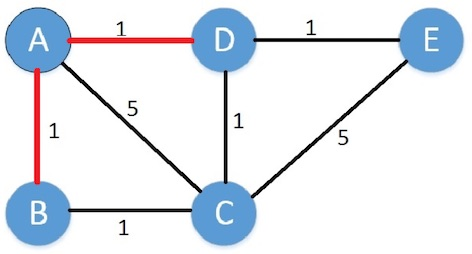
\includegraphics[width=0.4\textwidth]{tex/fig/Picture4}
	\caption{Trzeci etap wykonania algorytmu Kruskala}
	\label{fig: legendK3}
\end{figure}
\newpage
\item Krok 4\\
Ze zbioru S usunięta została jedna z krawędzi o najmniejszej wadze. {C D} Ponieważ wierzchołki, które łączyła znajdowały się w osobnych drzewach w L zostały połączone w jedno drzewo {A, B, C, D}, więc dodawana jest krawędź dodawana jest do W.\\
S: {A, B, C, D}, {E}
\\
L: {D E}, {B C}, {A C}, {C E}
\\

\begin{figure}[htb!]
	\centering
	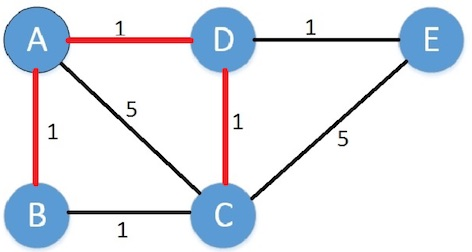
\includegraphics[width=0.4\textwidth]{tex/fig/Picture5}
	\caption{Czwarty etap wykonania algorytmu Kruskala}
	\label{fig: legendK4}
\end{figure}

\item Krok 5\\
Ze zbioru S usunięta została jedna z krawędzi o najmniejszej wadze. {D E} Ponieważ wierzchołki, które łączyła znajdowały się w osobnych drzewach w L zostały połączone w jedno drzewo {A, B, C, D, E}, więc dodawana jest krawędź dodawana jest do W. Ponieważ w zbiorze L pozostał tylko jeden zbiór wykonanie algorytmu zostaje zakończone.\\
S: {A, B, C, D, E}
\\
L: {B C}, {A C}, {C E}
\\
\begin{figure}[htb!]
	\centering
	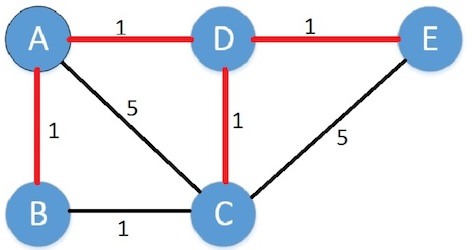
\includegraphics[width=0.4\textwidth]{tex/fig/Picture6}
	\caption{Piąty etap wykonania algorytmu Kruskala – uzyskane MST}
	\label{fig: legendK5}
\end{figure}

\textbf{Jak widać nie zawiera ono żadnych cykli i zawiera tylko krawędzie o minimalnej wadze.}\\
\end{enumerate}
\newpage
\subsection{Opis struktur danych i algorytmów}
\begin{itemize}
		\item Dane zostaną pobrane z pliku tekstowego o ustalonym formacie.
		\item Ponieważ samodzielna implementacja podstawowych algorytmów mija się z celem użyta zostanie jedna z funkcji bibliotecznych języka JAVA.
		\item Wykrywanie cykli oraz scalanie odbywać się będzie poprzez użycie struktury zbiorów rozłącznych - \cite{gis2}.
		\item Krawędzie dodane do grafu będą wpisywane do listy w celu zapisania uzyskanego rozwiązania.
\end{itemize}

\section{Opis wybranych struktur danych}
Aby uzyskać taką samą złożoność czasową dla obu wybranych algorytmów (\emph{O(E$\cdot$ log V)}), obrano następujące założenia: 
\begin{itemize}
	\item Implementacja algorytmu Prima jest oparta na kolejce priorytetowej, w której operacja wstawiania elementu ma złożoność \emph{O(logn)}, gdzie n, to liczba elementów w kolejce.
	\item Implementacja algorytmu Kruskala jest oparta na listowej implementacji struktury zbiorów rozłącznych.
\end{itemize}

\begin{center}
\textbf{Aby zrealizować ten cel, wykorzystano w implementacji obu algorytmów następujące struktury danych:}
\end{center}

\subsection{Stos}
Stos jest strukturą danych, z której elementy są odczytywane w kolejności odwrotnej do ich wstawiania. Struktura ta nosi nazwę LIFO. Rozróżniamy następujące operacje dla stosu:
\begin{itemize}
	\item sprawdzenie, czy stos jest pusty – operacja \textbf{empty} zwraca true, jeśli  stos nie zawiera żadnego elementu, w przeciwnym razie zwraca false
	\item odczyt szczytu stosu – operacja \textbf{top} zwraca element (zwykle jest to wskaźnik) znajdujący się na szczycie stosu, sam element pozostaje wciąż na stosie
	\item zapis na stos – operacja \textbf{push} umieszcza na szczycie stosu nowy element
	\item usunięcie ze stosu – operacja \textbf{pop} usuwa ze szczytu stosu znajdujący się tam element
\end{itemize}

Stos krawędzi w implementacji algorytmu Prima reprezentuje minimalne drzewo rozpinające - MST i krawędzie są jedynie do niego dodawane metodą \textbf{push}.\\

\newpage
\subsection{Kolejka priorytetowa}
Kolejka priorytetowa jest kolejką, w której elementy są ułożone nie w kolejności wprowadzania, lecz w kolejności priorytetu. Każdy element kolejki posiada dodatkowe pole \emph{prio}, w którym przechowuje swój priorytet – czyli ważność. Gwarantuje to pobieranie z kolejki jako pierwszych elementów o najwyższym priorytecie. Elementy o priorytetach niższych zostaną pobrane dopiero wtedy, gdy zostaną usunięte wszystkie elementy o priorytetach wyższych.\\
W implementacji algorytmu Prima rolę \emph{prio} pełni waga krawędzi.\\
W niniejszym projekcie operacje \textbf{empty}, \textbf{front} i \textbf{pop} niczym się nie różnią od takich samych operacji dla zwykłej kolejki. Jedyna różnica pojawia się przy operacji \emph{push}, która umieszcza w kolejce nowy element. W tym przypadku lista jest przeglądana od początku do końca, aby znaleźć w niej krawędź o wadze bezpośrednio wyższej od wagi dodawanej krawędzi. Przed znalezioną krawędzią zostaje dodana nowa krawędź.\\

\subsection{Tablica}
Tablica, to kontener danych takiego samego typu, gdzie każdy z elementów jest dostępny za pomocą klucza zwanego indeksem. W implementacji algorytmu Prima, tablica \emph{visitedVertices} reprezentuje odwiedzone wierzchołki grafu i jest to tablica jednowymiarowa.\\

\newpage
\section{Założenia programu i ogólny projekt testów}
\begin{enumerate}
	\item Algorytmy zostaną wykonane dla \textbf{grafów spójnych, nieskierowanych}.
	\item Wszystkie pomiary zostaną wykonane na następującej maszynie:\\
	-- MacBook Air z procesorem 1,7 GHz Intel Core i7\\
	\item Porównaniu ulegnie czas wykonywania obu algorytmów.
	\item Oba algorytmy zostaną wykonane dla grafów o określonej liczbie wierzchołków oraz krawędzi.
	\item Pomiar czasu będzie wykonywany od momentu oznaczającego pierwszy krok każdego z algorytmów aż do wykonania ostatniej istrukcji z ostatniego kroku.
	\item Pomiar czasu będzie wykonywany w około 1000 iteracjach, a następnie ulegnie uśrednieniu. Schemat poglądowy programu podczas pomiaru czasu wygląda następująco:\\
	
	\begin{figure}[htb!]
		\centering
		
\includegraphics[width=0.5\textwidth]{tex/fig/time}
		\caption{Zarys pomiaru czasu podczas wykonywania algorytmu}
		\label{fig: time}
	\end{figure}

\end{enumerate}
Dokładna liczba iteracji zostanie dobrana metodą prób i błędów podczas wykonywania pomiarów.
\chapter{Przebieg badań}
\fancyhead[C]{PRZEBIEG BADAŃ}
\fancyhead[L]{}
\fancyhead[R]{}

\section{Obrane założenia}
\begin{enumerate}
	\item Przez wzgląd na duży rozmiar wygenerowanych grafów wybranych do wykonania projektu, w celu przeprowadzenia obliczeń wykorzystano\textbf{ MacBook Pro z procesorem  Intel Core i7-6820HQ oraz 16 GB pamięci RAM}.
	\item Minimalna liczba iteracji, wystarczająca do wykonania badań, to \textbf{100}, jednak przez wzgląd na możliwości sprzętowe, zdecydowano się na liczbę iteracji równą \textbf{1000}.
	\item Badania przeprowadzono dla grafów o \textbf{liczbie wierzchołków} równej: 10, 50, 100, 500, 1000, 5000 oraz 10 000.
	\item Badania przeprowadzono dla grafów o \textbf{gęstości} równej: 0.2, 0.4, 0.6, 0.8 oraz 1.0.
\end{enumerate}

\newpage
\section{Przebieg obliczeń}
Aby określić liczbę iteracji, przeprowadzono testy na grafie pełnym o 1000 wierzchołkach. Wyniki tych badań prezentuje tabela \ref{fig: tab1}.

\begin{figure}[htb!]
	\centering
	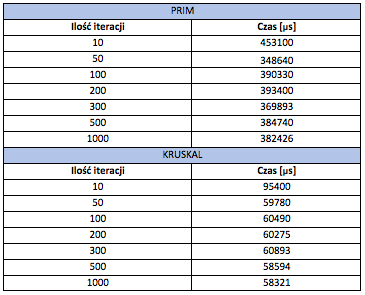
\includegraphics[width=0.5\textwidth]{tex/fig/tab1}
	\caption{Wyniki badań czasu wykonania algorytmów dla różnej liczby iteracji.}
	\label{fig: tab1}
\end{figure}
%%%%%%%%%%%%%%%%%%%%%%%%%%%%%%%%%%%%%%%%%%%%%%%%%%%%%%%%%%%%%%%%%%%%%%%%%%%%%%%%%%%%%%%%%%%%%%%%%%%%%%%%%%%%%%%%%%%%%%%%

Z tabeli \ref{fig: tab1} wynika, że minimalną liczbą iteracji dla prowadzonych obliczeń jest liczba 100, ponieważ  wartości czasu wykonania algorytmu dla większych od niej liczb iteracji niewiele się od siebie różnią. \textbf{Jednak dzięki dostępnym możliwościom sprzętowym zdecydowano się na ustawienie liczby iteracji równej 1000.}
%%%%%%%%%%%%%%%%%%%%%%%%%%%%%%%%%%%%%%%%%%%%%%%%%%%%%%%%%%%%%%%%%%%%%%%%%%%%%%%%%%%%%%%%%%%%%%%%%%%%%%%%%%%%%%%%%%%%%%%%
\newpage
Następnie obliczono liczbę krawędzi dla grafów o danej liczbie wierzchołków oraz zakładanej gęstości. Wyniki obliczeń, zarazem zbiór danych grafów wejściowych, prezentuje tabela \ref{fig: tab2}.

\begin{figure}[htb!]
	\centering
	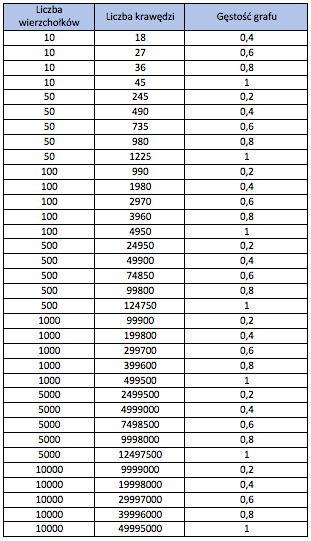
\includegraphics[width=0.5\textwidth]{tex/fig/tab2}
	\caption{Dane niezbędne do wygenerowania grafu o określonych parametrach.}
	\label{fig: tab2}
\end{figure}

\newpage 
Po ustawieniu liczby iteracji w programie, przystąpiono do wykonania obliczeń w następujący sposób:
\begin{enumerate}
	\item Wygenerowano graf o zadanych parametrach.
	\item Po wygenerowaniu grafu uruchomiono algorytm Prima.
	\item Po wykonaniu wszystkich iteracji dla algorytmu Prima, uruchomiono algorytm Kruskala.
\end{enumerate}


\subsection{Weryfikacja poprawności implementacji algorytmów}
Algorytmy zostały przetestowane na grafach dla których znane jest poprawne MST. Następnie porównane zostały wyniki obu algorytmów dla pewnych grafów losowych. 
Podczas wszystkich przeprowadzonych testów liczone i porównywane były nie tylko zbiory krawędzi tworzących MST, ale również sumy wag tych krawędzi.

Wstępne obliczenia dla grafu pełnego o 1000 wierzchołkach wykazały dużą rozbieżność pomiędzy wynikami czasu wykonania dla obu algorytmów (na niekorzyść Prima). 
Wpływ na zaistniałą sytuację miały następujące czynniki:
\begin{enumerate}
	\item Niewłaściwy sposób pomiaru czasu dla algorytmu Kruskala - pominięto sortowanie  krawędzi na początku algorytmu.
	\item Struktura reprezentująca graf -- algorytm Prima zoptymalizowano dzięki wykorzystaniu do tego celu list sąsiedztwa (zamiast macierzy sąsiedztwa).
\end{enumerate}

Wyniki przeprowadzonych obliczeń zaprezentowano w sekcji \ref{results}.
\newpage
\section{Wyniki eksperymentu}
\label{results}
Po dokonaniu optymalizacji i poprawy zaistniałych niedociągnięć wykonano obliczenia, których wyniki zestawiono w tabeli \ref{fig: tab3}.
\begin{figure}[htb!]
	\centering
	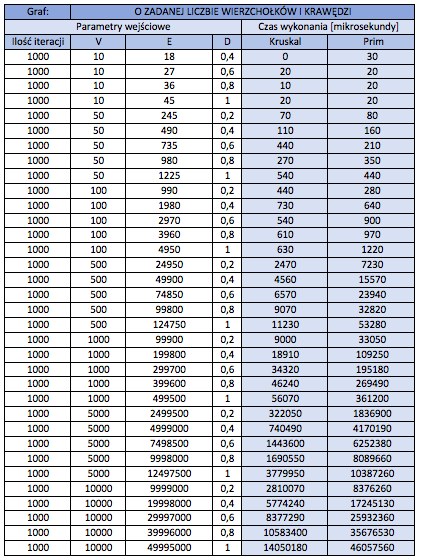
\includegraphics[width=0.8\textwidth]{tex/fig/tab3}
	\caption{Wyniki obliczeń dla obu algorytmów.}
	\label{fig: tab3}
\end{figure}

\newpage
Otrzymane wyniki przedstawiono również w formie wykresów:
\begin{itemize}
 \item Zależność czasu wykonania algorytmu Prima od gęstości D danych grafów prezentuje wykres \ref{fig: w1}. 
 
 \begin{figure}[htb!]
 	\centering
 	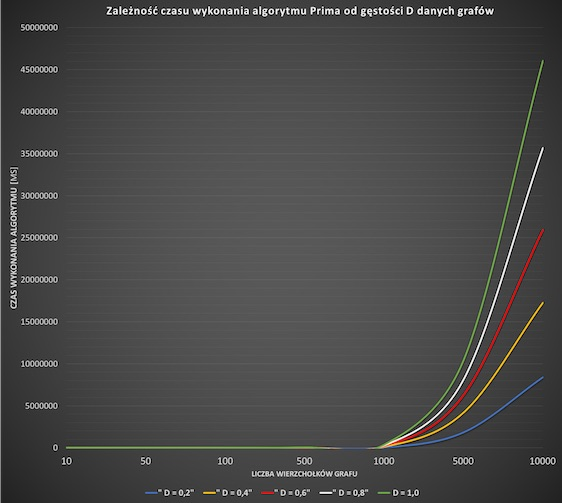
\includegraphics[width=1 \textwidth]{tex/fig/p1}
 	\caption{Zależność czasu wykonania algorytmu Prima od gęstości D danych grafów.}
 	\label{fig: w1}
 \end{figure}

\newpage
 Wykres ten został też podzielony na dwie części w celu zwiększenia czytelności:
 \begin{enumerate}
 	\item Zależność czasu wykonania algorytmu Prima od gęstości grafów o liczbie wierzchołków V$\subseteq$\{10,50,100,500,1000\} - rys. \ref{fig: ww1}
 	
 	 \begin{figure}[htb!]
 		\centering
 		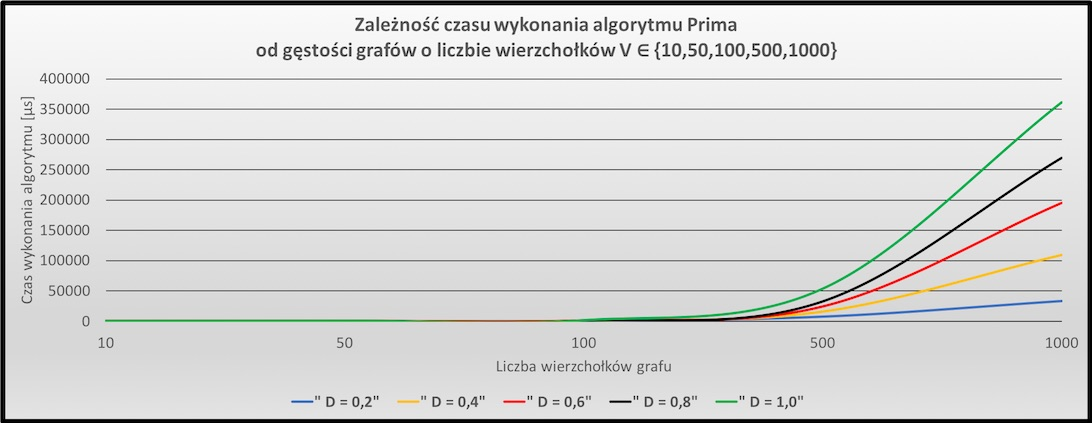
\includegraphics[width=1\textwidth]{tex/fig/p2_10_1000}
 		\caption{Zależność czasu wykonania algorytmu Prima od gęstości grafów o liczbie wierzchołków V$\subseteq$ \{10,50,100,500,1000\}}
 		\label{fig: ww1}
 	\end{figure}
 
 	\item Zależność czasu wykonania algorytmu Prima od gęstości grafów o liczbie wierzchołków V$\subseteq$ \{500,1000,5000,10000\} - rys. \ref{fig: ww11}.
 	
 	 \begin{figure}[htb!]
 		\centering
 		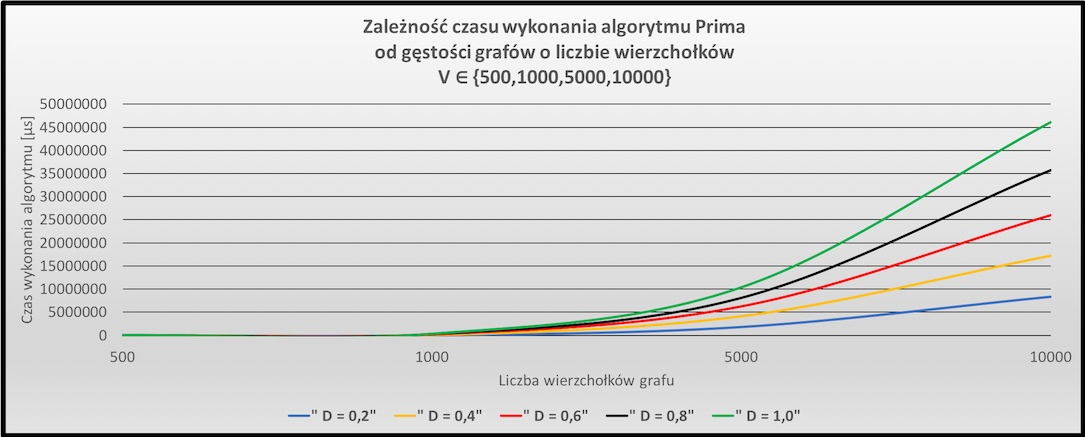
\includegraphics[width=1\textwidth]{tex/fig/p22}
 		\caption{Zależność czasu wykonania algorytmu Prima od gęstości grafów o liczbie wierzchołków V$\subseteq$ \{500,1000,5000,10000\} } 
 		\label{fig: ww11}
 	\end{figure}
 
 \end{enumerate}
\newpage
 \item Zależność czasu wykonania algorytmu Kruskala od gęstości D danych grafów prezentuje wykres \ref{fig: w2}. 
 
  \begin{figure}[htb!]
 	\centering
 	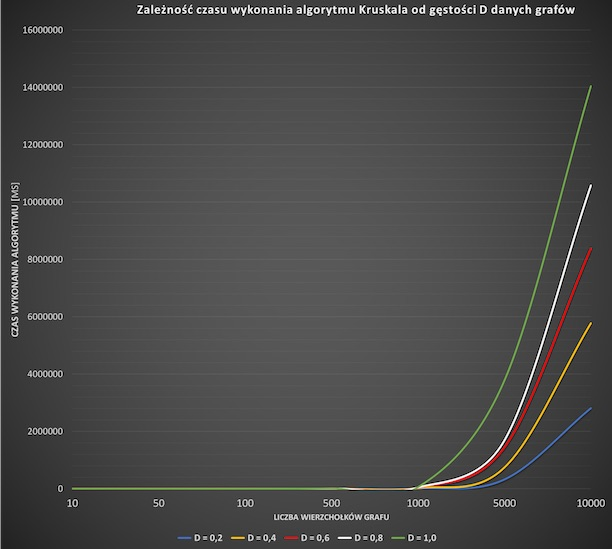
\includegraphics[width=1\textwidth]{tex/fig/k1}
 	\caption{Zależność czasu wykonania algorytmu Kruskala od gęstości D danych grafów.}
 	\label{fig: w2}
 \end{figure}

\newpage
 Wykres ten został też podzielony na dwie części w celu zwiększenia czytelności:
  \begin{enumerate}
 	\item Zależność czasu wykonania algorytmu Kruskala od gęstości grafów o liczbie wierzchołków V$\subseteq$ \{10,50,100,500,1000\}- rys. \ref{fig: ww2}
 	
\begin{figure}[htb!]
	\centering
	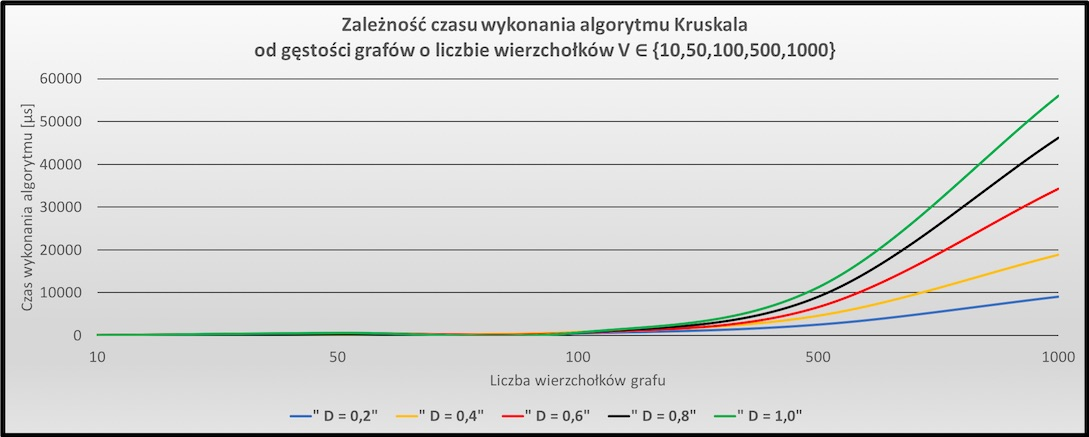
\includegraphics[width=1\textwidth]{tex/fig/k2_10_1000}
	\caption{Zależność czasu wykonania algorytmu Kruskala od gęstości grafów o liczbie wierzchołków V$\subseteq$ \{10,50,100,500,1000\}}
	\label{fig: ww2}
\end{figure}

 	\item Zależność czasu wykonania algorytmu Kruskala od gęstości grafów o liczbie wierzchołków V$\subseteq$ \{500,1000,5000,10000\}  - rys. \ref{fig: ww2}.
 	
 	\begin{figure}[htb!]
 		\centering
 		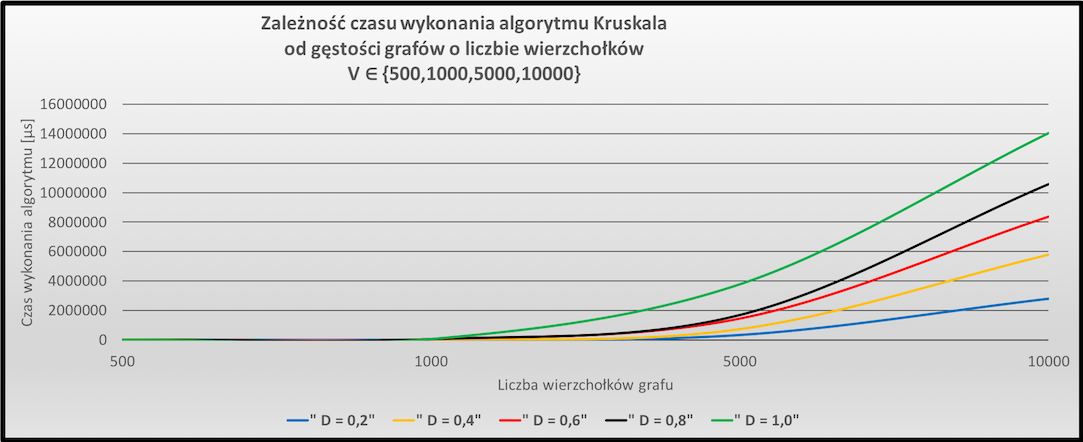
\includegraphics[width=1\textwidth]{tex/fig/k22}
 		\caption{Zależność czasu wykonania algorytmu Kruskala od gęstości grafów o liczbie wierzchołków V$\subseteq$ \{500,1000,5000,10000\} }
 		\label{fig: ww22}
 	\end{figure}
 \end{enumerate}

\item Zestawienie czasów wykonania algorytmów Prima i Kruskala dla grafów o zadanych parametrach z kolei prezentuje rys. \ref{fig: pk1}.
	\begin{figure}[htb!]
	\centering
	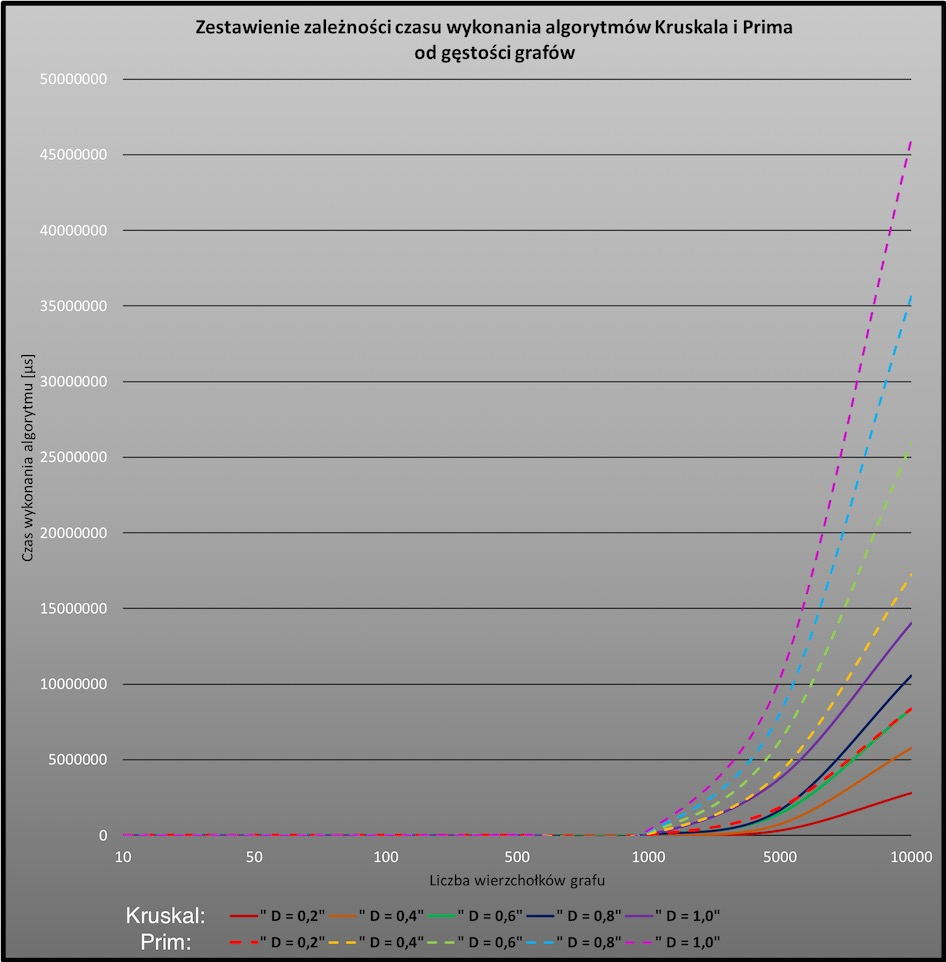
\includegraphics[width=1\textwidth]{tex/fig/kp1}
	\caption{Zestawienie zależności czasów wykonania algorytmów Prima i Kruskala od gęstości grafów}
	\label{fig: pk1}
\end{figure}
\newpage
Diagram ten jest podstawą dla wniosków wysuniętych w sekcji \ref{conclusion}. Dla poprawy czytelności podzielono go na dwie części:
\begin{enumerate}
	\item Zestawienie zależności czasu wykonania algorytmów Kruskala i Prima od gęstości grafów o liczbie wierzchołków V$\subseteq$ \{10,50,100,500,1000\} - rys. \ref{fig: kp1}.
	
		\begin{figure}[htb!]
		\centering
		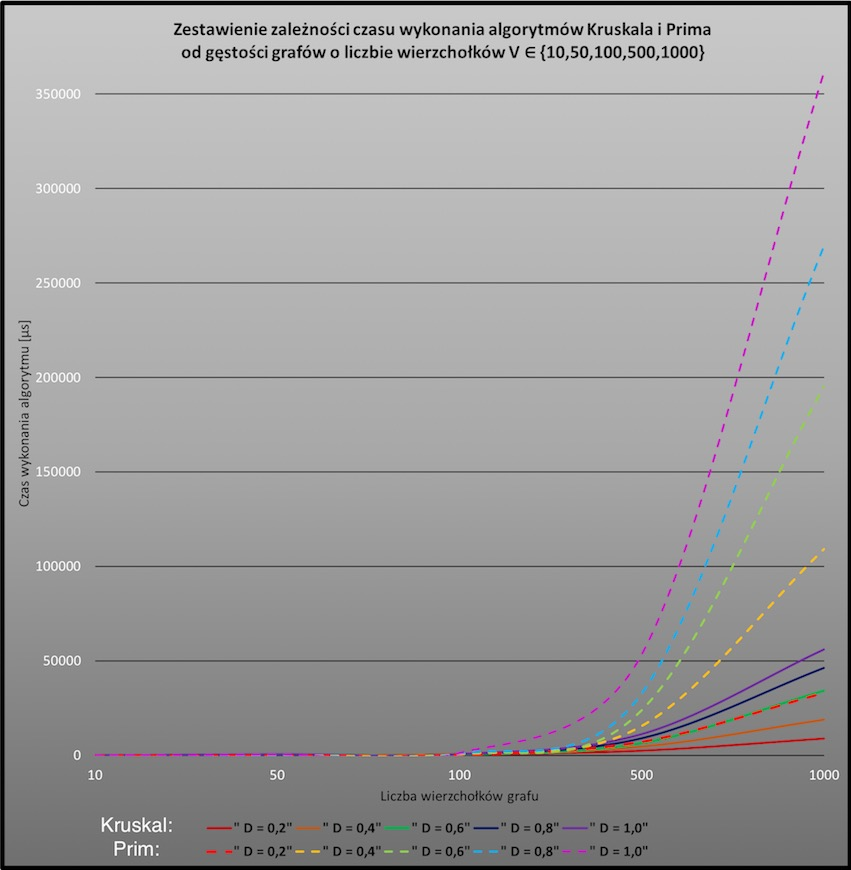
\includegraphics[width=1\textwidth]{tex/fig/kp_10_1000}
		\caption{Zestawienie zależności czasu wykonania algorytmów Kruskala i Prima od gęstości grafów o liczbie wierzchołków V$\subseteq$ \{10,50,100,500,1000\}}
		\label{fig: kp1}
	\end{figure}

\item Zestawienie zależności czasu wykonania algorytmów Kruskala i Prima od gęstości grafów o liczbie wierzchołków V$\subseteq$ \{500,1000,5000,10000\}  - rys. \ref{fig: kp2}.
\begin{figure}[htb!]
	\centering
	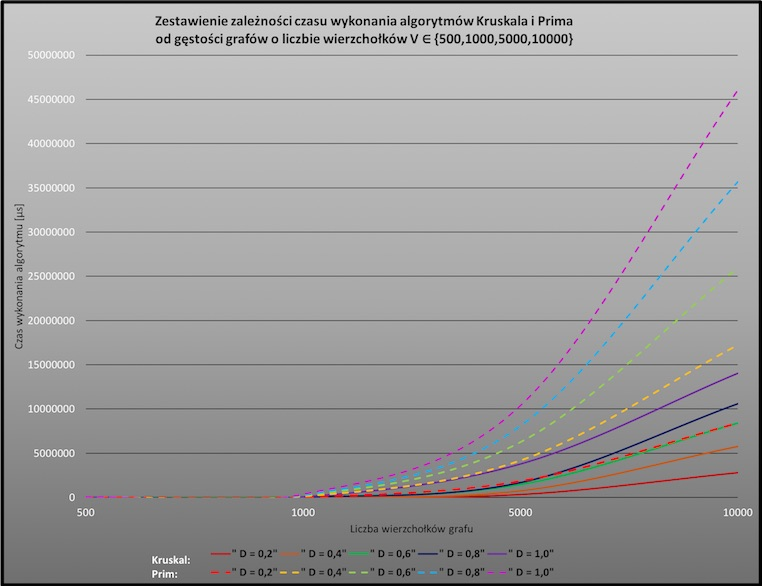
\includegraphics[width=1\textwidth]{tex/fig/kp_500_1000}
	\caption{Zestawienie zależności czasu wykonania algorytmów Kruskala i Prima od gęstości grafów o liczbie wierzchołków V$\subseteq$ \{500,1000,5000,10000\} }
	\label{fig: kp2}
\end{figure}
\end{enumerate}
\end{itemize}

\newpage
\section{Wnioski}
\fancyhead[C]{WNIOSKI}
\fancyhead[L]{}
\fancyhead[R]{}
\label{conclusion}
Na podstawie powyższych wyników obliczeń wyciągnięto następujące wnioski:
\begin{enumerate}
	\item Dla małych grafów algorytm Prima uzyskuje porównywalne (a nawet lepsze) wyniki względem algorytmu Kruskala
	\item W przypadku dużych grafów zastosowanie algorytmu Kruskala sprawdza się lepiej przez wzgląd na krótszy czas wykonywania 
	\item Z diagramu wynika, że algorytm Prima ma dłuższy czas wykonywania od algorytmu Kruskala
	\item W przypadku grafów o małej gęstości algorytm Kruskala radzi sobie znacznie lepiej od algorytmu Prima
	\item Różnice czasu wykonywania algorytmu wynikają z:\\
	-- Implementacji każdego z algorytmów\\
	-- Wykorzystanych do implementacji struktur danych\\
	-- Doboru odpowiednich parametrów generowanego do obliczeń grafu
\end{enumerate}



\setcounter{secnumdepth}{-1}

\chapter{Spis załączników}
\setcounter{secnumdepth}{3}

\setcounter{section}{0}
\renewcommand{\thesection}{\arabic{section}}
\newcommand{\CDlitera}{$\Xi$/}

\section{Kod źródłowy algorytmu Prima}
\section{Kod źródłowy modułu odpowiedzialnego za odczyt macierzy z pliku}
\section{Link do repozytorium z kodem źródłowym generatora macierzy sąsiedztwa}
\begin{center}
	\emph{https://github.com/joannasia9/Gis-pro}
\end{center}
%\section{Kod źródłowy algorytmu Kruskala}

%Usuwa numeracje z naglowka. Zapewnia  dodanie do spisu tresci

%Gdy mamy dużą bibliografię to możemy wybierać pozycje,
%które cytujemy
%\nocite{ad-tg-80}

%Dodaje wszystkie pozycje z bibliografii
%\nocite{*}

%Po kazdym dodaniu nowej pozycji bibliograficznej
%z katalogu glownego uruchom: bibtex pracadyp
%\bibliographystyle{pdplain}
%\bibliography{tex/pracadyp}

\listoffigures
\setcounter{secnumdepth}{-1}
\begin {thebibliography}{11}
\fancyhead[R]{BIBLIOGRAFIA}
\bibitem{prim} \emph{http://www.algorytm.org/algorytmy-grafowe/algorytm-prima.html}
\bibitem{prim2}\emph{http://algorytmika.wikidot.com/mst}
\bibitem{gis}Jacek Wojciechowski, Krzysztof Pieńkosz: \emph{Grafy i sieci},  Wydawnictwo Naukowe PWN SA, Warszawa 2013
\bibitem{gis2} \emph{http://www.ams.org/proc/1956-007-01/S0002-9939-1956-0078686-7/}
\end {thebibliography}


%\newpage
\fancyhead[C]{ZAŁĄCZNIKI}
\fancyhead[L]{}
\fancyhead[R]{}
\begin{center}
	\textbf{Załącznik 1.} Kod źródłowy algorytmu Prima
\end{center}

\begin{lstlisting}
	public class PrimAlgorithm{
	/**
	* Element losowosci
	*/
	Random rand;
	/**
	* Lista odwiedzonych wierzcholkow
	*/
	private ArrayList<Integer> visitedVertices;
	
	/**
	* Lista wszystkich wierzcholkow
	*/
	private ArrayList<Edge> adjacencyEdgesList;
	
	
	/**
	* Konstruktor
	* Odpowiada za wykonanie poszczegolnych krokow algorytmu
	*
	* @param  graph  macierz sasiedztwa reprezentujaca graf
	*
	*/
	public PrimAlgorithm(final int[][] graph){
	this.adjacencyEdgesList = new ArrayList<>();
	
	this.visitedVertices = new ArrayList<>();
	
	/**
	* Zbior krawedzi
	* Reprezentuje minimalne drzewo rozpinajace
	*/
	Set<Edge> minSpanningTree = new HashSet<>();
	
	/**
	* Zmienna pomocnicza
	* Lista krawedzi
	* Reprezentuje krawedzie incydentne do odwiedzonych wierzcholkow grafu
	*/
	ArrayList<Edge> adjacencyEdges;
	
	/**
	* Zmienna pomocnicza
	* Element odpowiedzialny za losowy wybor wierzcholka poczatkowego
	*/
	this.rand = new Random();
	
	/**
	* Losowy wybor wierzcholka poczatkowego
	* Z zakresu od 0 do n-1,
	* gdzie n-liczba wierzcholkow grafu
	*/
	int startV = rand.nextInt(graph.length-1);
	
	/**
	* Oznaczenie wierzcholka startowego jako odwiedzony
	* Dodanie wierzcholka startV do listy odwiedzonych wierzcholkow
	*/
	setVertexVisited(startV,visitedVertices);
	
	
	/**
	* Pobranie do zmiennej adjacencyEdges listy krawedzi incydentnych do startV
	*/
	adjacencyEdges = getAllAdjacencyEdges(startV,graph, adjacencyEdgesList);
	
	/**
	* Petla warunkowa while()
	* Wykonuje sie dopoki lista odwiedzonych wierzcholkow visitedVertices
	* nie zawiera wszystkich wierzcholkow grafu
	*/
	while(visitedVertices.size()!= graph.length) {
	/**
	* Zmienna reprezentujaca krawedz z listy krawedzi incydentnych
	* do punktow odwiedzonych adjacencyEdges, ktora ma minimalna wage
	*/
	Edge minEdge = adjacencyEdges.get(0);
	/**
	* Instrukcja warunkowa if()
	* Pod warunkiem, ze lista odwiedzonych wierzcholkow visitedVertices
	* nie zawiera wierzcholka koncowego krawedzi minEdge:
	*
	* Do MST zostaje dodana krawedz minEdge
	* Wierzcholek startV zmienia wartosc na wierzcholek koncowy minEdge
	* Krawedz minEdge zostaje usunieta z listy krawedzi incydentnych
	* do rozpatrzenia
	* Lista krawedzi incydentnych adjacencyEdges zostaje zaktualizowana 
	* o krawedzie
	* incydentne do wierzcholka startV
	*
	* W przeciwnym wypadku:
	* Krawedz minEdge zostaje usunieta z listy krawedzi do rozpatrzenia
	*/
	if(!visitedVertices.contains(minEdge.getEnd())){
	minSpanningTree.add(minEdge);
	setVertexVisited(minEdge.getEnd(), visitedVertices);
	startV = minEdge.getEnd();
	adjacencyEdges.remove(minEdge);
	adjacencyEdges = getAllAdjacencyEdges(startV,graph,adjacencyEdgesList);
	} else adjacencyEdges.remove(minEdge); 	}
	/**
	* Wypisanie otrzymanego MST w konsoli
	*/
	printMST(minSpanningTree); }
	/**
	* @param vertex
	* @param list
	* Oznacza wierzcholek jako odwiedzony poprzez dodanie wierzcholka vertex
	* do listy wierzcholkow odwiedzonych list
	*/
	private void setVertexVisited(int vertex, ArrayList<Integer> list){
	/**
	* Instrukcja warunkowa if()
	* Blok instrukcji zostaje wykonany, gdy lista wierzcholkow odwiedzonych 
	* nie zawiera jeszcze wierzcholka vertex
	*/
	if(!list.contains(vertex))
	list.add(vertex);
	}
	
	/**
	*
	* @param vertex
	* @param graph
	* @return
	*
	* Dodaje do listy adjacencyEdgesList krawedzie incydentne 
	* do wierzcholka vertex, ktore nie tworza cyklu
	*/
	private ArrayList<Edge> getAllAdjacencyEdges(int vertex, 
										int[][] graph, ArrayList<Edge> adjacencyEdgesList){
	
	/**
	* Instrukcja iteracyjna for()
	* Blok instrukcji jest wykonywany dla kazdego wierzcholka grafu
	*/
	for(int i=0; i<graph.length; i++){
	/**
	* Instrukcja warunkowa if()
	* Operacja dodania krawedzi incydentnej do wierzcholka vertex 
	* zostaje wykonana pod warunkiem, ze:
	* Krawedz (vertex-i) istnieje, czyli jej waga jest rozna od 0 oraz
	* Lista odwiedzonych wierzcholkow visitedVertices 
	* nie zawiera jeszcze i-tego wierzcholka
	*/
	if(graph[vertex][i]!= 0 && !visitedVertices.contains(i))
			adjacencyEdgesList.add(new Edge(vertex,i,graph[vertex][i]));
	}
	
	/**
	* Sortowanie otrzymanej listy krawedzi wzgledem wag
	*/
	Collections.sort(adjacencyEdgesList);
	
	return adjacencyEdgesList;
	}
	
	/**
	*
	* @param set
	*
	* Wyswietla w konsoli liste krawedzi otrzymanego drzewa
	* wraz z suma wag krawedzi
	*/
	private void printMST(Set<Edge> set){
	int sum = 0;
	for(Edge item : set){
	System.out.println(item);
	sum+=item.getWeight();
	}
	System.out.println("SUMA WAG WYNOSI: " + sum);
	}
\end{lstlisting}


\begin{center}
	\textbf{Załącznik 1.a.} Kod źródłowy klasy Edge
\end{center}

\begin{lstlisting}
	/**
	* Klasa Edge, ktorej obiekty reprezentuja krawedzie grafu
	*/
	private class Edge implements Comparable<Edge> {
	/**
	* Wierzcholek poczatkowy krawedzi
	*/
	private int start;
	/**
	* Wierzcholek koncowy krawedzi
	*/
	private int end;
	/**
	* Waga krawedzi (start - end)
	*/
	private int weight;
	
	/**
	*
	* @param s
	* @param e
	* @param w
	*
	* Konstruktor krawedzi
	*/
	Edge(int s, int e, int w){
	setStart(s);
	setEnd(e);
	setWeight(w);
	}
	
	private int getWeight(){
	return weight;
	}
	
	private int getStart() {
	return start;
	}
	
	private void setStart(int start) {
	this.start = start;
	}
	
	private int getEnd() {
	return end;
	}
	
	private void setEnd(int end) {
	this.end = end;
	}
	
	private void setWeight(int weight) {
	this.weight = weight;
	}
	
	/**
	*
	* @param e
	* @return
	* Metoda odpowiedzialna za porownywanie krawedzi
	* Wykorzystywana podczas sortowania krawedzi w liscie
	* @see Collections
	*/
	@Override
	public int compareTo(Edge e) {
	if (getWeight() < e.getWeight()){
	return -1;
	} else if (getWeight() > e.getWeight()) {
	return 1;
	}
	return 0;
	}
	
	/**
	* @return
	*
	* Metoda odpowiedzialna za postac wypisanej w konsoli krawedzi
	*/
	@Override
	public String toString() {
	return String.format("%d--%d\tw:%d ", start, end, weight);
	}
	}
\end{lstlisting}
\newpage
\begin{center}
	\textbf{Załącznik 2.} Kod źródłowy modułu odpowiedzialnego za odczyt macierzy z pliku
\end{center}

\begin{lstlisting}
	import java.io.*;
	
	public class GraphFileExtractor {
	private Graph graph;
	private int[][] adjacencyMatrix;
	
	public void getFileContent(int iterator) {
	String home = System.getProperty("user.home");
	File file = new File(home + File.separator + "Desktop" 
											+ File.separator + "G" + iterator + ".txt");
	
	try {
	BufferedReader br = new BufferedReader(new FileReader(file.getPath()));
	String line = br.readLine();
	initiateMatrix(line);
	
	int i = 0;
	while (line != null) {
	parseLine(i,line);
	line = br.readLine();
	i+=1;
	}
	
	} catch (IOException e) {
	e.printStackTrace();
	}
	}
	
	private void parseLine(int i, String line){
	String delim = "\t";
	String[] tokens = line.split(delim);
	
	for(int j=0; j<tokens.length;j++){
	if(Integer.parseInt(tokens[j])!=0)
	graph.addEdge(new Edge(i,j,Integer.parseInt(tokens[j])));
	adjacencyMatrix[i][j] = Integer.parseInt(tokens[j]);
	}
	
	}
	
	private void initiateMatrix(String line){
	String delim = "\t";
	String[] tokens = line.split(delim);
	graph = new Graph(tokens.length);
	adjacencyMatrix = new int[tokens.length][tokens.length];
	}
	
	public Graph getGraph(){
	return graph;
	}
	
	public int[][] getAdjacencyMatrix(){
	return adjacencyMatrix;
	}
	}
\end{lstlisting}

\end{document}
